% VUT FIT 3BIT
% ISA 2018/2019
% Project: Programming Network Service
% Author: Vladimir Dusek, xdusek27
% Date: 30/9/2018
% File: isa-assignment.tex

%%%%%%%%%%%%%%%%%%%%%%%%%%%%%%%%%%%%%%%%%%%%%%%%%%%%%%%%%%%%%%%%%%%%%

\documentclass[11pt, a4paper, titlepage]{article}
\usepackage[left=2cm, text={17cm, 24cm}, top=3cm]{geometry}
\usepackage[utf8]{inputenc}
\usepackage[czech]{babel}
\usepackage{pdfpages}
\usepackage[obeyspaces]{url}
\usepackage{framed}
\usepackage[T1]{fontenc}
\usepackage{lmodern}
\usepackage[thinlines]{easytable}
\usepackage{float}

\setlength\parindent{0pt}

%%%%%%%%%%%%%%%%%%%%%%%%%%%%%%%%%%%%%%%%%%%%%%%%%%%%%%%%%%%%%%%%%%%%%

\begin{document}

\begin{titlepage}
	\begin{center}
		\begin{figure}[htb]
			\centering
			
\includegraphics[width=0.85\hsize]{fitlogo.pdf}
		\end{figure}
		\vspace{\stretch{0.382}}
		{\Huge Síťové aplikace a správa sítí} \\
		\bigskip
		{\LARGE Dokumentace k~projektu Programování síťové služby} \\
		\bigskip
		{\Large Varianta 2: Export DNS informací pomocí protokolu Syslog}
		\vspace{\stretch{0.618}}
	\end{center}
	{\Large \today \hfill Vladimír Dušek, xdusek27}
\end{titlepage}

%%%%%%%%%%%%%%%%%%%%%%%%%%%%%%%%%%%%%%%%%%%%%%%%%%%%%%%%%%%%%%%%%%%%%

\tableofcontents
\newpage

%%%%%%%%%%%%%%%%%%%%%%%%%%%%%%%%%%%%%%%%%%%%%%%%%%%%%%%%%%%%%%%%%%%%%

\section{Úvod}

Dokumentace popisuje řešení projektu a vysvětluje danou problematiku. Naší úlohou bylo nastudovat si potřebné informace a následně navrhnout, naprogramovat a otestovat síťovou službu, navíc k ní napsat manuálovou stránku. Varianta 2, kterou jsem řešil spočívala ve vytvoření aplikace dns-export. Ta odposlouchává síťový provoz na síťovém rozhraní, případně zpracovává pcap soubor, ve kterém je nějaká síťová komunikace již zaznamenána. Aplikace vyfiltruje DNS provoz a následně zpracovává jednotlivé pakety, konkrétně DNS odpovědi (responses). V každé odpovědi projde skrz všechny odpovědní záznamy (Answer resource records) a vyčte určité informace. Doménové jméno, typ DNS záznamu a data specifická pro každý typ. Dále je zaznamenán výskyt těchto informací, shodné jsou sečteny. Tyto výsledky jsou zasílany na syslog server ve formátu odpovídající syslog protokolu.

\newpage

%%%%%%%%%%%%%%%%%%%%%%%%%%%%%%%%%%%%%%%%%%%%%%%%%%%%%%%%%%%%%%%%%%%%%

\section{Uvedení do problematiky}

\subsection{Model TCP/IP}

Síťová komunikace je kvůli své komplexnosti rozdělena do tzv. vrstev, které znázorňují hierarchii činností. Výměna informací mezi vrstvami je přesně definována. Každá vrstva využívá služeb vrstvy nižší a poskytuje své služby vrstvě vyšší.

\subsubsection{Vrstva síťového rozhraní}

Nejnižší vrstva, umožňuje přístup k fyzickému médiu. Je specifická pro každou síť v závislosti na její implementaci. (např. Ethernet)

\subsubsection{Síťová vrstva}

Vrstva zajišťuje síťovou adresaci, směrování a předávání datagramů. Je implementována ve všech prvcích sítě -- směrovačích i koncových zařízeních. (např. IPv4, IPv6, ARP, ICMP)

\subsubsection{Transportní vrstva}

Poskytuje transportní služby pro kontrolu celistvosti dat. Jedná se o spolehlivé spojení (TCP) nebo nespolehlivé spojení (UDP). Je implementována až v koncových zařízeních, proto umožňuje přizpůsobit chování sítě potřebám aplikace.

\subsubsection{Aplikační vrstva}
Vrstva, která se stará o přenos konkrétních aplikačních dat. (např. SSH, FTP, HTTP, DHCP, DNS)

\begin{figure}[htp]
    \centering
    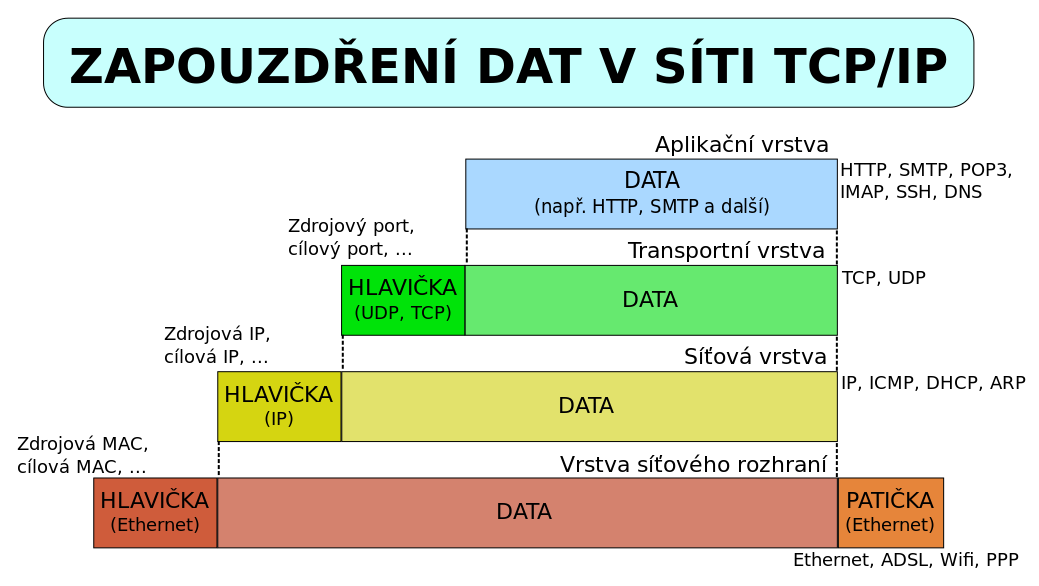
\includegraphics[width=.55\textwidth]{layers_schema.png}\hfill
    \caption{Schéma zapouzdření dat na vrstvách TCP/IP}
\end{figure}

\subsection{Domain Name System}

DNS (Domain Name System) je hierarchický systém doménových jmen, který je realizován servery DNS a protokolem stejného jména, kterým si vyměňují informace. Jeho hlavním úkolem jsou vzájemné převody doménových jmen a IP adres sítě. Slouží de facto jako distribuovaná databáze síťových informací.

\subsubsection{Formát DNS zprávy}

DNS zpráva má následující formát:

\begin{table}[H]
	\centering
	\begin{TAB}(r,3cm,0.75cm)[5pt]{|c|}{|c|c|c|c|c|}
		Header \\
		Question \\
		Answer \\
		Authority \\
		Additional \\
	\end{TAB}
\end{table}

Header (hlavička) blíže specifikuje DNS zprávu. Například zda se jedná o dotaz, či odpověď, zda nastala nějaká chyba, nebo kolik zpráva obsahuje DNS záznamů (resource records) a jakých jsou typů. \\

V sekci Question (dotaz) jsou informace které chce tázající zjistit. Konkrétně doménové jméno na které se dotazuje, typ a třída záznamu. \\

Answer, Authority a Additional jsou pak záznamy. Všechny mají shodný formát a obsahují různé odpovědi, případně cestu jak se odpovědí dosáhlo.

\subsection{Syslog protokol}

Syslog protokol je standard pro záznam programových zpráv (logů). Program podle protokolu posílá zprávy napříč sítí ke kolektorům logovacích zpráv -- syslog serverům. Jedná se tedy o architekturu klient-server. Komunikace může probíhat přes UDP na portu 514 nebo přes TCP na portu 6541.

\subsubsection{Formát zpráv}

Maximální délka paketu je 1024 bytů. Zpráva má následující formát:

\begin{center}
	\fbox{PRI HEADER MSG}
\end{center}

Část PRI se skládá ze třech až pěti znaků. Začíná znakem '<', následuje číslo a končí znakem '>'. Číslo uvnitř špičatých závorek se nazývá Priority value a reprezentuje Facility -- zařazení podsystému a Severity -- míru závažnosti.

\begin{center}
	\fbox{PRI = <Priority Value>} \\
\end{center}

Priority value se vypočítá následujícím vzorcem:

\begin{center}
	\fbox{Priority Value = Facility * 8 + Severity}
\end{center}

Část HEADER obsahuje časovou značku -- TIMESTAMP, tedy kdy byla zpráva odeslána a adresu odesílatele -- HOSTNAME, tedy kdo zprávu odeslal.

\begin{center}
	\fbox{HEADER = TIMESTAMP HOSTNAME} \\
\end{center}

Poslední část, MSG, se sestává opět ze dvou částí. První z nich je TAG, což je název procesu, který zprávu vygeneroval a druhá je CONTENT, tedy konkrétní obsah zprávy.

\begin{center}
	\fbox{MSG = TAG CONTENT} \\
\end{center}

\newpage

%%%%%%%%%%%%%%%%%%%%%%%%%%%%%%%%%%%%%%%%%%%%%%%%%%%%%%%%%%%%%%%%%%%%%

\section{Struktura programu}

Aplikace se snaží držet objektově orientovaného paradigma. Kvůli spravování signálů (signal handler) bylo nutné některé věci definovat na globální úrovni.
\smallskip

Jako první se pracuje s instancí třídy ArgParser, která se stará o zpracování argumentů příkazové řádky a jejich validaci. Argumenty jsou uloženy jako privátní atributy a přístup k nim je definován pomocí příslušných metod.
\smallskip

Třída PcapParser využívá pcap knihovnu pro odchytávání síťového provozu na síťovém zařízení, případně pro parsování zdrojového pcap souboru. Dále vyfiltruje DNS provoz a zpracuje veškeré hlavičky až k aplikační vrstvě. Poradí si na síťové vrstvě s IPv4 i IPv6 datagramama a na transportní vrstvě s TCP i UDP komunikací.
\smallskip

Třída DnsParser zpracovává data DNS protokolu. Vytřídí pouze odpovědi (responses), které neskončili chybou. Projde všechny záznamy v sekci Answers a vybere data potřebná k vytvoření statistik. Statistiky ukládá do globální datové struktury unordered map jako dvojice klíč->hodnota. Klíč jsou získaná data z DNS záznamu a value je počet výskytů těchto dat za celou dobu odchytávání, případně za zpracování celého pcap souboru.
\smallskip

Třída Syslog se pak stará o komunikaci se syslog serverem. Poskytuje metody pro připojení, odpojení a odesílání zpráv na syslog.
\smallskip

Ve funkci signal handler jsou pak odchytávány signály, SIGUSR1 pro výpis statistik na STDOUT, SIGALRM pro odeslání statistik na syslog server a SIGINT pro ukončení aplikace (v případě odposlouchávání na síťovém rozhraní běží aplikace až do obdržení tohoto signálu).

\newpage

%%%%%%%%%%%%%%%%%%%%%%%%%%%%%%%%%%%%%%%%%%%%%%%%%%%%%%%%%%%%%%%%%%%%%

\section{Implementace}

...

\newpage

%%%%%%%%%%%%%%%%%%%%%%%%%%%%%%%%%%%%%%%%%%%%%%%%%%%%%%%%%%%%%%%%%%%%%

\section{Testování}

...

\newpage

%%%%%%%%%%%%%%%%%%%%%%%%%%%%%%%%%%%%%%%%%%%%%%%%%%%%%%%%%%%%%%%%%%%%%

\section{Použití}

...

\newpage

%%%%%%%%%%%%%%%%%%%%%%%%%%%%%%%%%%%%%%%%%%%%%%%%%%%%%%%%%%%%%%%%%%%%%

\section{Dodatečné informace}

...

\newpage

%%%%%%%%%%%%%%%%%%%%%%%%%%%%%%%%%%%%%%%%%%%%%%%%%%%%%%%%%%%%%%%%%%%%%
\end{document}
